
\chapter{Trigonometrie}

Die Trigonometrie ist eigentlich ein Teilgebiet der Geometrie. Da wir in diesem Buch aber keinen Geometrie Teil haben, wird dieses durchaus wichtige Thema in der Analysis behandelt. 

\section{Differentialgleichung}

Betrachten wir die folgende Differentialgleichung:
\begin{equation}\label{eq:diffsincos}
f''(x) + f(x) =0
\end{equation}
wir suchen also Funktionen, deren zweite Ableitung gerade das Negative ihrer selbst sind. Versuchen wir doch einmal eine Reihe aufzuschreiben, die diese Bedingung erfüllt. Finden wir eine solche Reihe, dann ist diese eine Lösung der Differentialgleichung. Eine Lösung zu einer Differentialgleichung zu raten ist ein probates Mittel. Denn raten wir korrekt, ist dies die Lösung, denn gewöhnliche Differentialgleichungen haben nur eine Lösung.

Wir wissen aus der Ableitung von Polynomen, dass die zweite Ableitung eines Monoms die folgende ist:

\begin{equation}
\left(a_0 + a_2\cdot x^2 + a_4 \cdot x^4 \right)'' = a_2 + a_4 \cdot 4\cdot 3 \cdot x^2
\end{equation}
wählen wir $a_0=1$, $a_2 = \frac{-a_0}{2}=-\frac{1}{2}$ und $a_4 = \frac{-a_2}{4\cdot 3}= \frac{1}{4\cdot 3\cdot 2}$, so gilt 

\begin{equation}
\left(1 - \frac{1}{2}x^2 + \frac{1}{4\cdot 3\cdot 2} x^4 \right)'' = -1 +\frac{1}{2}x^2
\end{equation}
Auf diese Weise bekommen wir sehr einfach eine Funktion, bei der wir die einzelnen Monome so zusammenbauen, dass ihre zweite Ableitungen gerade das negative des vorhergehenden Monoms ergibt. Führen wir dann diese Reihe weiter fort, so ergibt sich
\begin{equation}
\left( 1-\frac{1}{2!}x^2 +\frac{1}{4!}x^4 -\frac{1}{6!}x^6+\frac{1}{8!}x^8 \pm \dots \right)'' =
-1+\frac{1}{2!}x^2 -\frac{1}{4!}x^4 +\frac{1}{6!}x^6 -\frac{1}{8!}x^8 \pm \dots
\end{equation}
Als Summe geschrieben:
\begin{equation}
c(x) = \sum_{i=0}^{\infty} (-1)^{i} \cdot \frac{1}{(2i)!} x^{2i}
\end{equation}
Wir haben so durch Überlegung eine Funktion gefunden, die eine Lösung der Differentialgleichung (\ref{eq:diffsincos}) ist. Denn es gilt
\begin{equation}
c''(x) +c(x) = 0
\end{equation}
Betrachten wir zusätzlich noch die erste Ableitung von $c$, sie ist aufgrund unserer Wahl der Faktoren sehr einfach zu berechnen:
\begin{equation}
c'(x) = \sum_{i=1}^{\infty} (-1)^{i}\cdot \frac{1}{(2i-1)!}x^{2i-1}
\end{equation}
Aufgrund dessen, dass $c''(x) = -c(x)$ gilt, ist auch $c'''(x) = -c'(x)$. Wir wählen uns einen Funktionsnamen $s$ derart, dass $c'(x) = -s(x)$ ist. Es ist
\begin{equation}
s(x) = \sum_{i=0}^{\infty} (-1)^i \cdot \frac{1}{(2i+1)!}x^{2i+1}
\end{equation}
Dann ist $s'(x) = c(x)$ und $c'(x) = -s(x)$. Und $s$ erfüllt, genau wie $c$
\begin{equation}
s''(x) +s(x) =0
\end{equation}
Wir haben also zwei Lösungen zu einer Differentialgleichung. Die Tatsache, dass die $s$ Funktion nur aus ungeraden Exponenten zu $x$ besteht und $c$ nur aus geraden Exponenten zu $x$ lässt uns vermuten, dass $s$ und $c$ linear unabhängige Funktionen sind. In den Aufgaben wird dies nachgewiesen. Vorher muss natürlich noch bestimmt werden, dass $s$ und $c$ Elemente eines Funktionenraums sind. Genauer sind sie Elemente des $C^{\infty}$, des Raumes aller unendlich oft differenzierbaren Funktionen. Mit dem Skalarprodukt des $C^\infty$ gilt
\begin{equation}
\langle s,c\rangle = 0
\end{equation}

Die Namen $s$ und $c$ unserer Funktionen sind natürlich nicht zufällig so gewählt, dies sind gerade die Sinus ($s$) und Cosinus ($c$) Funktionen. Abbildung 

\begin{figure}[h]
\centering
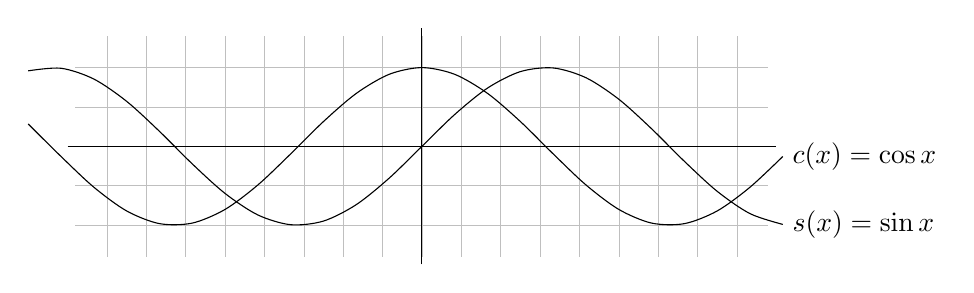
\begin{tikzpicture}
\draw[step=.5cm,lightgray,very thin] (-4.4,-1.4) grid (4.4,1.4);
\draw (-4.5,0) -- (4.5,0);
\draw (0,-1.5) -- (0,1.5);

\draw[color=black]   plot[smooth] (\x,{sin(\x r)})    node[right] {$s(x) = \sin x$};
\draw[color=black]   plot[smooth] (\x,{cos(\x r)})    node[right] {$c(x) = \cos x$};
  
\end{tikzpicture}
\caption{Die Sinus und Kosinus Funktionen}
\end{figure}

 

\section{Taylor-Reihe}

